\documentclass[12pt]{article}
\usepackage{listings}
\usepackage{amssymb}
\usepackage{amsthm}
\usepackage{amsmath}
\usepackage{graphicx}
\usepackage{subfig}
\usepackage{multirow}
\usepackage{float}
\usepackage{fancyhdr}
\usepackage{caption, subcaption}
\usepackage{tabularx}
\usepackage{booktabs}
\usepackage{multicol}
\usepackage{array}
\usepackage{adjustbox}
\usepackage[cache=false]{minted}
\usepackage{xcolor}
\usepackage[font=small]{caption}
\usepackage{siunitx}
\usepackage{subfigure}
\usepackage{subcaption}
\usepackage{graphicx} % Include this line in the preamble
\usepackage{pgfplots}
\pgfplotsset{compat=1.17}

\definecolor{bg}{rgb}{1.0, 0.97, 0.7} % Light yellow

\setminted[c]{
  bgcolor=bg,
  linenos,
  fontsize=\footnotesize,
  breaklines
}

\captionsetup{compatibility=false}
\usepackage[hidelinks, colorlinks=true, linkcolor=black, urlcolor=blue, citecolor=red]{hyperref}
%margin settings
\usepackage[left=2.5cm, right=2.5cm, top=4cm, bottom=3cm, footskip=0.5cm]{geometry}
% suppressing page numbers
\renewenvironment{abstract}
{\quotation
  {\large\bfseries\abstractname\centering\par\noindent\rule{\linewidth}{.5pt}\medskip}
  \noindent}
{\par\noindent\rule{\linewidth}{.5pt}\endquotation}

% Make headers
\usepackage{fancyhdr}
\pagestyle{fancy}
\fancyhf{}
\fancyhfoffset[L]{1cm} % left extra length
\fancyhfoffset[R]{1cm} % right extra length
\rhead{Group: 1}
\lhead{HW 05: Parallelization of 2-Dimensional Wave Equation with MPI}
\fancyfoot[C]{\thepage}


\lstset{frame=tb,
  language=C,
  aboveskip=3mm,
  belowskip=3mm,
  showstringspaces=false,
  columns=flexible,
  basicstyle={\small\ttfamily},
  numbers=none,
  numberstyle=\tiny\color{red},
  keywordstyle=\color{blue},
  commentstyle=\color{green},
  stringstyle=\color{red},
  breaklines=true,
  breakatwhitespace=true,
  tabsize=3
}
\title{ME 489 Homework 05 \\ Parallelization of 2-Dimensional Wave Equation with MPI}
\date{\today}
\author{Enes Çağlar Korkmazgöz 2370567 - Hasan Kaan Özen 2378586}

\begin{document}
\maketitle

\begin{abstract}
This report presents a code using a message passing interface in 2-dimensional wave equation solver parallelize. Strong scaling analysis and speedups are presented and discussed. The results show that as the code is parallelized, the run-time reduces significantly up to a certain point. This limit is depicted in the strong-scaling analysis, where the domain size is kept constant whilst the number of processes increases. Moreover, different grid sizes for resolution analysis are presented, and a mesh-independence study is done. It is shown that domain discretization for each process affects the error, yielding dependency on the mesh size.
\end{abstract}
\newpage
\tableofcontents
\newpage
\section{Introduction}

\noindent
Parallel computing helps reduce the total run-time in a C-written program. This yields reducing the computational costs and saving money to the user especially when the problem size is large enough and not feasible for a serial solver. In such a parallelization procedure, one may use OpenMP or MPI to utilize different processes in the solution algorithm; however, it was shown in Homework 04 [1] that MPI is more advantageous over OpenMP in terms of time reduction capability. So, in this report, the steps of implementing an MPI in an explicit in-time,  2-dimensional wave Equation \ref{eq:1} are presented, followed by results of total run times and scaling analysis. The findings are then discussed and interpreted.


\begin{equation}
\label{eq:1}
\frac{\partial^2 q}{\partial t^2} = c^2 \left( \frac{\partial^2 q}{\partial x^2} + \frac{\partial^2 q}{\partial y^2} \right), \quad 0 \leq x \leq 1, \quad 0 \leq y \leq 1
\end{equation}
%%%%%%%%%%%%%%%%%%%%%%%%%%%%%%%%%%%%%

\section{Understanding The Solver}
\label{sec:2}
 The solver is an explicit in-time solver that initializes the field variable according to initial and boundary conditions. These initial and boundary conditions are obtained from the exact solution provided in the code. Then, for the discretization method, central differencing is applied to solve the field variable at the next time step. The central differencing method for the discretization of time and space is presented in Equation \ref{eq:2}, Equation \ref{eq:3}, and Equation \ref{eq:4}, respectively.
\begin{align}
\label{eq:2}
\frac{\partial^2 q}{\partial t^2} &\approx \frac{q(x, y, t + \Delta t) - 2q(x, y, t) + q(x, y, t - \Delta t)}{\Delta t^2} \\
\label{eq:3}
\frac{\partial^2 q}{\partial x^2} &\approx \frac{q(x + \Delta x, y, t) - 2q(x, y, t) + q(x - \Delta x, y, t)}{\Delta x^2} \\
\label{eq:4}
\frac{\partial^2 q}{\partial y^2} &\approx \frac{q(x, y + \Delta y, t) - 2q(x, y, t) + q(x, y - \Delta y, t)}{\Delta y^2}
\end{align}

\noindent
In the discretized version of the time and the domain terms, it may be seen that there are three different time values involved in the equations; these are the previous, current, and next time steps of the field variable $q$. Section \ref{sec:3} presents the procedure for applying these conditions.

\section{Implementation Details}
\label{sec:3}
\subsection{Domain Decomposition}
For the parallelization of a discrete equation, a domain decomposition is a mandatory step to assign every processor a domain to compute in. For the case of this report, the global domain is divided to equal parts on the vertical axis. The resulting domain size for each processor is presented in Equation \ref{size}, where NX is the global number of horizontal nodes, NY is the global number of vertical nodes. For this report, the division on the right-hand side is assumed to be an exact division. The implementation is presented below.
\begin{equation}
\label{size}
    N_{size} = NX*\frac{NY}{N_{processors}}
\end{equation}
    \begin{minted}[linenos,breaklines,bgcolor=bg]{c}
  int nx = NX;      // local number of nodes in x direction
  int ny = NY/size;      // local number of nodes in y direction
    \end{minted}
\subsection{Uniform Spacing}
The uniform space between each node has to be calculated to compute the coordinates of each node. The calculation is presented in Equations \ref{uniform} and \ref{uniform1}. In these equations, "hx" and "hy" refer to uniform spacings in the horizontal and vertical axes, and size refers to the number of processors assigned. In Equation \ref{uniform1}, the global vertical size, "ymax-ymin" is not divided by the global number of vertical nodes because although the exact division assumption is made for the calculation of the local number of vertical nodes, using "ny*size" corrects the spacing calculation for non-exact divisions. The implementation is presented below.
\begin{equation}
    \label{uniform}
    hx = \frac{x_{max}-x_{min}}{NX-1}
\end{equation}
\begin{equation}
    \label{uniform1}
    hx = \frac{y_{max}-y_{min}}{(ny*size)-1}
\end{equation}
    \begin{minted}[linenos,breaklines,bgcolor=bg]{c}
  // find uniform spacing in x and y directions
  // Correct uniform y spacing for the local number of nodes as it may be round value.
  double hx = (xmax - xmin)/(NX-1.0); 
  double hy = (ymax - ymin)/((ny*size)-1.0);
    \end{minted}
\subsection{Coordinate Calculation}
The coordinates of the nodes have to be calculated so that the exact solution and the boundary conditions can be calculated for each node since they depend on position. The horizontal and vertical position calculations for an arbitrary node (i,j) are presented in Equations \ref{positionx} and \ref{positiony}. It should be noted that the vertical position calculation contains a multiplication with "rank" on the right-hand side. This implementation is necessary for parallelization since we decomposed the domain on the vertical axis and the vertical position of every rank is the sum of the vertical size of the domains of previous ranks. The implementation is presented below.
\begin{equation}
    \label{positionx}
    x[i+j*nx] = x_{min} + i*hx
\end{equation}
\begin{equation}
    \label{positiony}
    y[i+j*nx] = y_{min} + j*hx + (rank*hy*ny)
\end{equation}
    \begin{minted}[linenos,breaklines,bgcolor=bg]{c}
  // Compute coordinates of the nodes
  // Compute y coordinates according to ranks
  for(int j=0; j < ny; ++j){ 
    for(int i=0; i < nx;++i){
      // Every processors vertical size is (rank*hy*ny). This is the MPI correction for vertical position.
      double xn = xmin + i*hx; 
      double yn = ymin + (j*hy) + (rank*hy*ny);
      x[i+j*nx] = xn; 
      y[i+j*nx] = yn;}}
    \end{minted}

\subsection{Memory Allocation and Calculating Initial Solution}
There are three different arrays to allocate memory for the solution of the wave equation. These are the solution at the next time step, "qn", the solution at the initial time step, "q0", and the solution at the previous time step, "q1". For a serial code, the required memory for these arrays are the domain size multiplied by the size of a "double" storage. However, for an MPI code, extra memory allocation for the communications between processors is a necessity. Consequently, the communication structure has to be formed in order to allocate correct memory to the arrays.
\subsubsection{MPI Communication Structure}
Since the problem works on a decomposed domain in the vertical axis, a row of shadow nodes at the size of "nx", the number of horizontal nodes, has to be added to the bottom and top rows of a domain. These rows will store values either from the next rank or the previous rank depending on the row so that central differencing can be calculated correctly. The communication structure is presented in Figure \ref{comms}.
\begin{figure}[H]
    \centering
    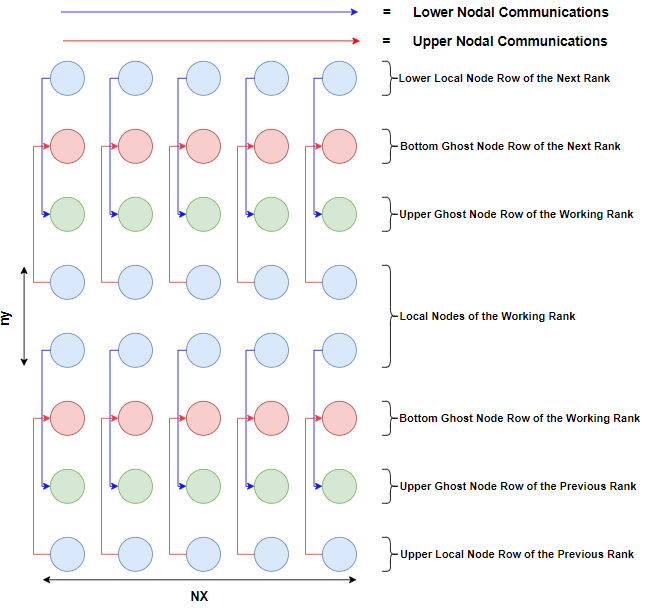
\includegraphics[scale=0.75]{hw5_comms_structure.png}
    \caption{MPI Communication Structure}
    \label{comms}
\end{figure}
With this communication structure, every rank will work on a field variable array with an extra size of "2*nx" which is directly equal to two extra rows added to the original local domain. The memory allocation implementation is presented below.
    \begin{minted}[linenos,breaklines,bgcolor=bg]{c}
  // ALLOCATE MEMORY for SOLUTION and its HISTORY
  // Create ghost nodes at the lower and upper y axes for MPI communications.
  // Solution at time (t+dt)
  qn = ( double * ) malloc ( ((nx*ny)+(2*nx)) * sizeof ( double ) );
  // Solution at time (t)
  q0 = ( double * ) malloc ( ((nx*ny)+(2*nx)) * sizeof ( double ) );
  // Solution at time t-dt
  q1 = ( double * ) malloc ( ((nx*ny)+(2*nx)) * sizeof ( double ) );
    \end{minted}
\subsubsection{Initial Solution}
The initial solution has to be calculated for every node except for the boundary nodes so that the necessary history points are acquired for central differencing. The implementation is presented below with the functions that are used. It should be noted that the field variable arrays have an "nx" added to the destination of the value. The reasoning behind it is to avoid any computation for the ghost nodes of a domain which are located in the first and last "nx" sized destination.
    \begin{minted}[linenos,breaklines,bgcolor=bg]{c}
  // USE EXACT SOLUTION TO FILL HISTORY
    for(int j=0; j < ny; ++j){ 
      for(int i=0; i < nx;++i){
        const double xn = x[i+j*nx]; 
        const double yn = y[i+j*nx]; 
        // Exact solutions at history tstart and tstart+dt
        q0[i+ (j*nx) + nx] = exactSoln(c, xn, yn, tstart + dt);  
        q1[i+ (j*nx) + nx] = exactSoln(c, xn, yn, tstart);
    }
  }
    \end{minted}
        \begin{minted}[linenos,breaklines,bgcolor=bg]{c}
double exactSoln( double c, double x, double y, double t){
  const double pi = 3.141592653589793; 
  double value = sin( 2.0*pi*( x - c*t));
  return value;
}    \end{minted}
\subsection{Boundary Condition}
The boundary condition for the problem of this report is directly equal to the exact solution function provided in the previous section. For a global domain size of "NX*NY", the boundaries of this domain will be the following:
\begin{itemize}
    \item Left Boundary: i = 0
    \item Right Boundary: i = NX-1
    \item Bottom Boundary: j = 0
    \item Top Boundary: j = NY-1
\end{itemize}
Since we have a decomposed domain in the vertical, the boundary condition function will need corrections such that only the ranks that contain the bottom and top boundaries will have boundary condition calculations for. There is no correction required for the left and right boundaries since all domains contain boundary nodes in these boundaries. The implementation detail is presented below.
        \begin{minted}[linenos,breaklines,bgcolor=bg]{c}
    // Apply Boundary Conditions i.e. at i, j = 0, i,j = nx-1, ny-1
    applyBC(q0, x, y, c, time, nx, ny, rank, size); 
    \end{minted}
        \begin{minted}[linenos,breaklines,bgcolor=bg]{c}
void applyBC(double *data,  double *x, double *y, double c, double time, int nx, int ny, int rank, int size){

  // Apply Boundary Conditions
  double xn, yn; 
  //Modfiy Boundary Condition loops according to domain decomposition and ranks.
  for(int j=0; j<ny;++j){ // left right boundaries i.e. i=0 and i=nx-1
    xn = x[0 + j*nx]; 
    yn = y[0 + j*nx];    
    data[j*nx + nx] = exactSoln(c, xn, yn, time); 

    xn = x[nx-1 + j*nx]; 
    yn = y[nx-1 + j*nx];    
    data[nx-1 + j*nx + nx] = exactSoln(c, xn, yn, time); 
  }

  for(int i=0; i< nx; ++i){ // top and  bottom boundaries i.e. j=0 and j=ny-1
    xn = x[i]; 
    yn = y[i];
    //Check if rank == 0 since it contains the lower boundary.
    if(rank==0){
      data[i + nx] = exactSoln(c, xn, yn, time);
    }
    xn = x[i+ (ny-1)*nx]; 
    yn = y[i+ (ny-1)*nx];
    //Check if rank == size -1 since it contains the upper boundary.
    if(rank==(size-1)){     
      data[i + nx + (ny-1)*nx] = exactSoln(c, xn, yn, time);
    }
  }
}
\end{minted}

\subsection{MPI Communication Implementation}
With the communication structure provided in Figure \ref{comms} covered, the implementation details can now be provided. For this implementation, the MPI functions, "MPI\_Send" and "MPI\_Recv" are used. These functions point to the destination of the first point in the upper or lower ghost/local row where the information will either be received at or sent by, respectively. Afterward, "nx" amount of elements will be sent or received such that it covers the information on the entire row of subject. The key point here is not using a loop to send information from point to point, ultimately saving total run time. The implementation detail is presented below.
        \begin{minted}[linenos,breaklines,bgcolor=bg]{c}
    //Set up Communications
    if (rank > 0) {
        // Send the bottom row of the current domain to the upper ghost row of the previous rank
        MPI_Send(&q0[nx], nx, MPI_DOUBLE, rank - 1, downcomms, MPI_COMM_WORLD);

        // Receive the upper row of the previous domain at the lower ghost row of the working rank
        MPI_Recv(&q0[0], nx, MPI_DOUBLE, rank - 1, uppercomms, MPI_COMM_WORLD, &status);
    }
    if (rank < size - 1) {
        // Send the upper row of the current domain to the lower ghost row of the next rank
        MPI_Send(&q0[nx + (nx * (ny - 1))], nx, MPI_DOUBLE, rank + 1, uppercomms, MPI_COMM_WORLD);

        // Receive the bottom row of the next domain at the upper ghost row of the working rank
        MPI_Recv(&q0[nx + (nx * ny)], nx, MPI_DOUBLE, rank + 1, downcomms, MPI_COMM_WORLD, &status);
    }
    \end{minted}
\subsection{Central Differencing}
With all the necessary implementations covered, the program continues with the central differencing stage. Because of the uniform spacing in time and space, the Equations \ref{eq:2}, \ref{eq:3},\ref{eq:4} reduce to Equation \ref{discrete}. With this equation in hand, the neighboring nodes have to be calculated for an arbitrary node " \textbf{[i + j*nx + nx]} ". The nx addition is necessary to avoid the bottom ghost row of a domain, which is not a local node and will only take part as the southern neighbor, " \textbf{[i + j*nx + nx - j*nx] }" and for the upper ghost row, " \textbf{[i + j*nx + nx + j*nx] }". The implementation details are presented below. It should be noted that the boundary nodes are avoided with if conditions such that central differencing will not be applied to these nodes since they depend on the in-time boundary condition.
\begin{equation}
\label{discrete}
q^{n+1}_{i,j} = 2q^n_{i,j} - q^{n-1}_{i,j} + \alpha_x (q^n_{i+1,j} - 2q^n_{i,j} + q^n_{i-1,j}) + \alpha_y (q^n_{i,j+1} - 2q^n_{i,j} + q^n_{i,j-1})
\end{equation}
\text{where } $\alpha_x = c^2\Delta t^2 / \Delta x^2$ \text{ and } $\alpha_y = c^2\Delta t^2 / \Delta y^2$.
\noindent

\begin{minted}[linenos,breaklines,bgcolor=bg]{c}
    // Update solution using second order central differencing in time and space
    for(int j=0; j < ny; ++j){
      for(int i=1; i < nx-1;++i){// exclude left and right boundaries
        const int n0   = i + j*nx + nx; 
        const int nim1 = i - 1 + j*nx + nx; // node i-1,j
        const int nip1 = i + 1 + j*nx + nx; // node i+1,j
        const int njm1 = i + (j-1)*nx + nx; // node i, j-1
        const int njp1 = i + (j+1)*nx + nx; // node i, j+1
        // update solution
        //Check if lower boundary
        if(rank == 0){
          if (n0 >= 2*nx){
            qn[n0] = 2.0*q0[n0] - q1[n0] + alphax2*(q0[nip1]- 2.0*q0[n0] + q0[nim1])
                                        + alphay2*(q0[njp1] -2.0*q0[n0] + q0[njm1]); 
          }
        }
        //Check if upper boundary
        else if(rank == size-1){
          if (n0 < (nx + nx*(ny-1))){
            qn[n0] = 2.0*q0[n0] - q1[n0] + alphax2*(q0[nip1]- 2.0*q0[n0] + q0[nim1])
                                        + alphay2*(q0[njp1] -2.0*q0[n0] + q0[njm1]); 
          }
        }
        else{ 
            qn[n0] = 2.0*q0[n0] - q1[n0] + alphax2*(q0[nip1]- 2.0*q0[n0] + q0[nim1])
                                        + alphay2*(q0[njp1] -2.0*q0[n0] + q0[njm1]);
        } 
      }
    }
    \end{minted}
After finding the solution at the next time step, a new loop is introduced to update the solution arrays. The implementation is presented below. Boundaries are avoided in this section aswell.
\begin{minted}[linenos,breaklines,bgcolor=bg]{c}
    // Update history q1 = q0; q0 = qn, except the boundaries
    for(int j=0; j < ny; ++j){ 
      for(int i=1; i < nx-1;++i){
        int n0   = i + j*nx + nx;
        //Check if lower boundary
        if(rank == 0){
          if (n0 >= 2*nx){
            q1[n0] = q0[n0]; 
            q0[n0] = qn[n0];
            }
        }
        //Check if upper boundary
        else if(rank == size-1){
          if (n0 < (nx + nx*(ny-1))){
            q1[n0] = q0[n0]; 
            q0[n0] = qn[n0];
            }
        }
        else{  
          q1[n0] = q0[n0]; 
          q0[n0] = qn[n0];
        }
      }
    } 
    \end{minted}
\subsection{Calculating Infinity Norm}
The infinity norm is an indicator that shows the maximum amount of difference between the simulation result and the exact solution. In this program, the infinity norm is calculated using the provided definition for every node in a loop, and updating the infinity norm if it is found higher than the previous node. Afterward, since every rank calculates it's infinity norm, the MPI function, MPI\_Reduce is used to read the infinity norms of all ranks and write the maximum of them to a variable named global infinity norm. The implementation details are presented below.
\begin{minted}[linenos,breaklines,bgcolor=bg]{c}
  // Compute Linf norm of error at tend
    double linf = 0.0; 
    for(int j=0; j < ny; ++j){ 
      for(int i=0; i < nx;++i){
         double xn = x[i+ j*nx]; 
         double yn = y[i+ j*nx]; 
         // solution and the exact one
         double qn = q0[i + j*nx + nx]; 
         double qe = exactSoln(c, xn, yn, time);  
         linf  = fabs(qn-qe)>linf ? fabs(qn -qe):linf;
          if (rank==1)
          {
            //printf("    Infinity norm of the error: %.4e %.8e at node %d  \n", qn, time, i+j*nx);
          }
       }
    }
    double global_linf = 0.0;
    MPI_Reduce(&linf, &global_linf, 1, MPI_DOUBLE, MPI_MAX, 0, MPI_COMM_WORLD);
    \end{minted}
    
\subsection{Printing the Results}
The code outputs the infinity norm of error, the total run-time as Wall Clock time, and the total number of processors used. The implementation is presented below.
\begin{minted}[linenos,breaklines,bgcolor=bg]{c}
  if(rank==0){
    printf ( "  Wall clock elapsed seconds = %f for %d number of processors.\n", global_time,size );
    printf("    Infinity norm of the error: %.4e %.8e \n", global_linf, time);
    \end{minted}
The code can be compiled and executed with the following steps:
\begin{itemize}
    \item \textbf{Compile:} mpicc -o wmpi wave2d\_mpi.c -lm
    \item \textbf{Run:} mpirun -np (number of processors) ./wmpi input.dat
\end{itemize}

\newpage
\section{Discussion and Results}
\subsection{Performance Measurements}

The performance measurements are carried out with both strong-scaling analyses and speedup analyses. These results are done by using different resolutions (namely, 400x400, 200x200, and 100x100 grids) and different number of processes. The hardware used to run the program is depicted in Table \ref{tab:spec}.
\begin{table}[H]
\centering
\caption{Processor Specs}
\label{tab:spec}
\begin{tabular}{lc}
\toprule
\textbf{Specification} & \textbf{Details} \\
\midrule
Product & Intel i7-12650H \\
Total Cores & 10 \\
Performance Cores & 6 \\
Efficient Cores & 4 \\
Total Threads & 16 \\
Base Frequency & 1 GHz\\
Max Turbo Frequency & 4.7 GHz \\
Cache & 24 MB \\
\bottomrule
\end{tabular}
\end{table}
\newpage
\subsubsection{Strong Scaling Study}
A strong scaling analysis is required to measure the efficiency of increasing the number of processes' effect on the solution time. This is done simply by measuring the wall clock time of different sets of process numbers and then comparing their speeds in a plot while the domain size is kept constant. Our analyses are carried out in three different domain sizes (100x100, 200x200, 400x400), and their results are presented in Figure \ref{fig:2}, Figure \ref{fig:3}, and Figure \ref{fig:4}, respectively.\\\\
It may be seen from the strong scaling analyses that increasing the number of processes increases the performance by reducing the wall clock time; however, after a $saturation\ point$, the increase in the number of processes does not yield better performance. This is due to the fact that as the number of processes increases in a program, the overall messaging procedure starts to dominate the wall clock time. Also, the wall clock time for a greater domain size still seems to decrease with a very small slope. This immediately shows that as the problem size is greater, an increase in the number of processes is required. 
\begin{figure}[h!]
\centering % This centers the figure
\begin{tikzpicture}
\begin{axis}[
    xlabel={Number of Processes},
    ylabel={Wall Clock Time (s)},
    grid=major
    % Removed the legend entries
    ]
    % Scatter plot points
    \addplot[only marks] coordinates {
    (10,3.32069)
    (8,3.2353)
    (6,3.5342)
    (4,4.5578)
    (2,8.4918)
    (1,14.689)
    };

    % Connecting points with a line
    \addplot[mark=none, red] coordinates {
    (10,3.32069)
    (8,3.2353)
    (6,3.5342)
    (4,4.5578)
    (2,8.4918)
    (1,14.689)
    };

\end{axis}
\end{tikzpicture}
\caption{Strong Scaling Analysis for the fixed domain : 100 x 100.}
\label{fig:2}
\end{figure}

\begin{figure}[H]
\centering
\begin{tikzpicture}
\begin{axis}[
    xlabel={Number of Processes},
    ylabel={Wall Clock Time (s)},
    grid=major
    ]
    % Scatter plot points for 200x200
    \addplot[only marks] coordinates {
    (10,11.6718)
    (8,11.94614)
    (6,13.2841)
    (4,17.5352)
    (2,32.957)
    (1,56.905)
    };

    % Connecting points with a line
    \addplot[mark=none, blue] coordinates {
    (10,11.6718)
    (8,11.94614)
    (6,13.2841)
    (4,17.5352)
    (2,32.957)
    (1,56.905)
    };

\end{axis}
\end{tikzpicture}
\caption{Strong Scaling Analysis for the fixed domain: 200 x 200.}
\label{fig:3}
\end{figure}

\begin{figure}[H]
\centering
\begin{tikzpicture}
\begin{axis}[
    xlabel={Number of Processes},
    ylabel={Wall Clock Time (s)},
    grid=major
    ]
    % Scatter plot points for 400x400
    \addplot[only marks] coordinates {
    (10,44.216443)
    (8,44.881)
    (6,51.807)
    (4,69.217)
    (2,132.51)
    (1,234.767)
    };

    % Connecting points with a line
    \addplot[mark=none, green] coordinates {
    (10,44.216443)
    (8,44.881)
    (6,51.807)
    (4,69.217)
    (2,132.51)
    (1,234.767)
    };

\end{axis}
\end{tikzpicture}
\caption{Strong Scaling Analysis for the fixed domain: 400 x 400.} 
\label{fig:4}
\end{figure}

\newpage
\subsubsection{Strong Scaling Speedup Study}

A strong scaling speedup study measures the parallelization performance by showing at what fold the number of processes increased the performance of a program. It is the sole result of time taken for a serial process divided by the parallel method with a given number of processes. Again, for the fixed domain sizes (100x100, 200x200, 400x400), the strong scaling speedup analyses are done, and the results are depicted in Figure \ref{fig:5}, Figure \ref{fig:6}, and Figure \ref{fig:7}.
\noindent
In Figure \ref{fig:5}, it seems that the speedup ratio increases up to 8 processes; however, after that point, a break-even occurs, and the speedup decreases. As the domain size is 100x100 and relatively small, the messaging between processes takes more time than the speedup supplied by these processes. As a result, the total run-time increases.

\begin{figure}[H]
\centering
\begin{tikzpicture}
\begin{axis}[
    xlabel={Number of Processes},
    ylabel={Speedup},
    grid=major
    ]
    % Scatter plot points for 100x100
    \addplot[only marks] coordinates {
    (10,4.423478253)
    (8,4.540228109)
    (6,4.156244695)
    (4,3.222826802)
    (2,1.729786382)
    (1,1)
    };

    % Connecting points with a line
    \addplot[mark=none, red] coordinates {
    (10,4.423478253)
    (8,4.540228109)
    (6,4.156244695)
    (4,3.222826802)
    (2,1.729786382)
    (1,1)
    };

\end{axis}
\end{tikzpicture}
\caption{Speedup Analysis for the fixed domain: 100 x 100.}
\label{fig:5}
\end{figure}
\newpage

\noindent
Figure \ref{fig:6} and Figure \ref{fig:7} show the strong scaling speedup analyses for domains 200x200 and 400x400. One may conclude from these plots that increasing process number increases the speedup; however, there is a bottleneck for both domains around process size ~9. Although for the case of the 100x100 domain, the speedup decreased after that point, for both 200x200 and 400x400, the speedup continuously increased with a small slope. 
\\\\\noindent
Moreover, one may see the speed increase in the 400x400 domain is greater than the 200x200 domain after the four processes implementation. The final result shows that for ten process implementations, the speedup crosses 5-fold for the 400x400 domain, whereas for the 200x200 domain, it stays below the 5-fold value. This can be noted as parallelization is more beneficial for high domain sizes.

\begin{figure}[H]
\centering
\begin{tikzpicture}
\begin{axis}[
    xlabel={Number of Processes},
    ylabel={Speedup},
    grid=major
    ]
    % Scatter plot points for 200x200
    \addplot[only marks] coordinates {
    (10,4.875426241)
    (8,4.763463345)
    (6,4.283692535)
    (4,3.245186824)
    (2,1.726643809)
    (1,1)
    };

    % Connecting points with a line
    \addplot[mark=none, blue] coordinates {
    (10,4.875426241)
    (8,4.763463345)
    (6,4.283692535)
    (4,3.245186824)
    (2,1.726643809)
    (1,1)
    };

\end{axis}
\end{tikzpicture}
\caption{Speedup Analysis for the fixed domain: 200 x 200.}
\label{fig:6}
\end{figure}


\begin{figure}[H]
\centering
\begin{tikzpicture}
\begin{axis}[
    xlabel={Number of Processes},
    ylabel={Speedup},
    grid=major
    ]
    % Scatter plot points for 400x400
    \addplot[only marks] coordinates {
    (10,5.309495384)
    (8,5.230877209)
    (6,4.531569093)
    (4,3.391753471)
    (2,1.771692702)
    (1,1)
    };

    % Connecting points with a line
    \addplot[mark=none, green] coordinates {
    (10,5.309495384)
    (8,5.230877209)
    (6,4.531569093)
    (4,3.391753471)
    (2,1.771692702)
    (1,1)
    };

\end{axis}
\end{tikzpicture}
\caption{Speedup Analysis for the fixed domain: 400 x 400.}
\label{fig:7}
\end{figure}

\subsubsection{Tabulated Data}
There are three tabulated data tables for the resolutions mentioned previously. They depict the communication world size, the run-time of each program, speedup ratios, and the infinite norm of the error.\\\\
There is an interesting fact about these data. As described in Section 3 the domain is divided in the y-direction into several processes available. This is done assuming that the y-length of the problem is divisible by the number of processes, i.e., the communication world size. However, when we used six processes, which cannot divide the domains of sizes 100x100, 200x200, and 400x400, the infinite norm of the error is increased at that instant. So, one may also be cautious about this division operation across processes.\\\\
We have also constructed a 300x300 domain divisible by the six processes to show this. The results are well-aligned with the output of the serial processor now. This can be seen in the Table \ref{tab:300by300}.

% Table for 100x100
\begin{table}[htbp]
\centering
\caption{Performance for Problem Size 100x100}
\begin{tabular}{@{} cccc @{}}
\toprule
Processes & Run-time & Speedup & Infinite Norm of Error\\
\midrule
10 & 3.32069 & 4.423478253 & 9.08e-4 \\
8 & 3.2353 & 4.540228109 & 9.0811e-4 \\
6 & 3.5342 & 4.156244695 & 9.0811e-4 \\
4 & 4.5578 & 3.222826802 & 9.0869e-4 \\
2 & 8.4918 & 1.729786382 & 9.0869e-4 \\
1 & 14.689 & 1 & 9.0869e-4 \\
\bottomrule
\end{tabular}
\end{table}

% Table for 200x200
\begin{table}[htbp]
\centering
\caption{Performance for Problem Size 200x200}
\begin{tabular}{@{} cccc @{}}
\toprule
Processes & Run-time & Speedup & Infinite Norm of Error\\
\midrule
10 & 11.6718 & 4.875426241 & 3.239e-4 \\
8 & 11.94614 & 4.763463345 & 3.239e-4 \\
6 & 13.2841 & 4.283692535 & 3.2513e-4 \\
4 & 17.5352 & 3.245186824 & 3.239e-4 \\
2 & 32.957 & 1.726643809 & 3.239e-4 \\
1 & 56.905 & 1 & 3.239e-4 \\
\bottomrule
\end{tabular}
\end{table}

% Table for 400x400
\begin{table}[htbp]
\centering
\caption{Performance for Problem Size 400x400}
\begin{tabular}{@{} cccc @{}}
\toprule
Processes & Run-time & Speedup & Infinite Norm of Error\\
\midrule
10 & 44.216443 & 5.309495384 & 2.1767e-4 \\
8 & 44.881 & 5.230877209 & 2.1767e-4 \\
6 & 51.807 & 4.531569093 & 2.1766e-4 \\
4 & 69.217 & 3.391753471 & 2.1767e-4 \\
2 & 132.51 & 1.771692702 & 2.1767e-4 \\
1 & 234.767 & 1 & 2.1767e-4 \\
\bottomrule
\end{tabular}
\end{table}

% Table for 300x300
\begin{table}[htbp]
\centering
\caption{Error for Problem Size 300x300}
\label{tab:300by300}
\begin{tabular}{@{} ccc @{}}
\toprule
Processes & Infinite Norm \\
\midrule
6  & 2.4363e-04 \\
1 & 2.4363e-04 \\

\bottomrule
\end{tabular}
\end{table}





%%%%%%%%%%%%%%%%%
\clearpage

\section{Conclusion}
In this project, we have implemented MPI to parallelize a 2-dimensional wave equation solver, which is explicit in time. The solver is first run in a serial processor, and then the implementation results of the MPI for the parallel solver are depicted in tables and figures. This implementation is time-consuming, especially compared to the OpenMP applications; however, the results show that this approach effectively reduces the run-time whilst preserving the results' accuracy. \\

\noindent
The application is based on the fact that MPI's distributed memory structure. Successful implementation of MPI then requires $shadow rows$ approach, as the domain is divided into sub-domains by splitting it in the y-direction. This is done by sending and receiving information on the node of interest (boundary/shadow nodes) to the next and previous ranks, respectively. This approach also requires a thorough calculation of the world size and the domain size, as it is assumed that the domain is divisible by the number of processes available.\\\\

\noindent
Measuring the performance of the different domains and process sizes is the report's main goal. So, a strong-scaling study is carried out to compare the results. Not only wall clock times but also speedups are compared, and it is concluded that as the domain size increases, the parallelization is more beneficial to the user, and as the processor number is increased, after a certain instant, the costs take over the benefit from the parallelization as the message passing between processes takes longer times to compute.\\\\

\noindent
Furthermore, saving energy is increasingly important in today's high-performance computing (HPC) systems. As you add more processes, it directly impacts how much power is used. Therefore, energy consumption is a key consideration when comparing MPI and OpenMP for decision-making.\\\\

\noindent
In conclusion, while MPI boasts superior scalability and flexibility in distributed environments, choosing a number of processes is another consideration as we do not have unlimited resources, and also unlimited resources (processes availability) do not always result in higher performances. Users should be informed of the task's specific requirements, including the problem's scale, the available hardware, and the desired balance between computational performance and energy efficiency to choose the number of processes.
\noindent

\newpage
\section{References}
[1] Korkmazgoz, Ozen, ME489 HW4 (2023).

\noindent
[2] Lecture notes of Ali Karakuş for ME489 (2023).


\end{document}